\documentclass[/Users/ikedahajime/GitHub/reserch/master_report/thesis]{subfiles}
% このファイル内だけのコマンド
\begin{document}
% \chapter{結果}
\section{壁の形状による影響}
この章では、壁の形状を変えたときの結果を示す。具体的には、壁の形状を1つの円から2つの円をつなげたものに変え、そのダイナミクスを見る。
TODO:ここに粒子はいち
\figref{fig:twocer_lo0.7_r10_m0.1}は、高密度の ABP 系における$\psi_2、V_2$
を、2円間の距離の関数としてプロットした図である。半径$R=10$、$\varphi=0.7、M=0.1$のパラメータを用いた。

\begin{figure}[htbp]
    \centering
    \begin{tabular}{c}
        \begin{minipage}{0.4\hsize}
            \text{(a)}
            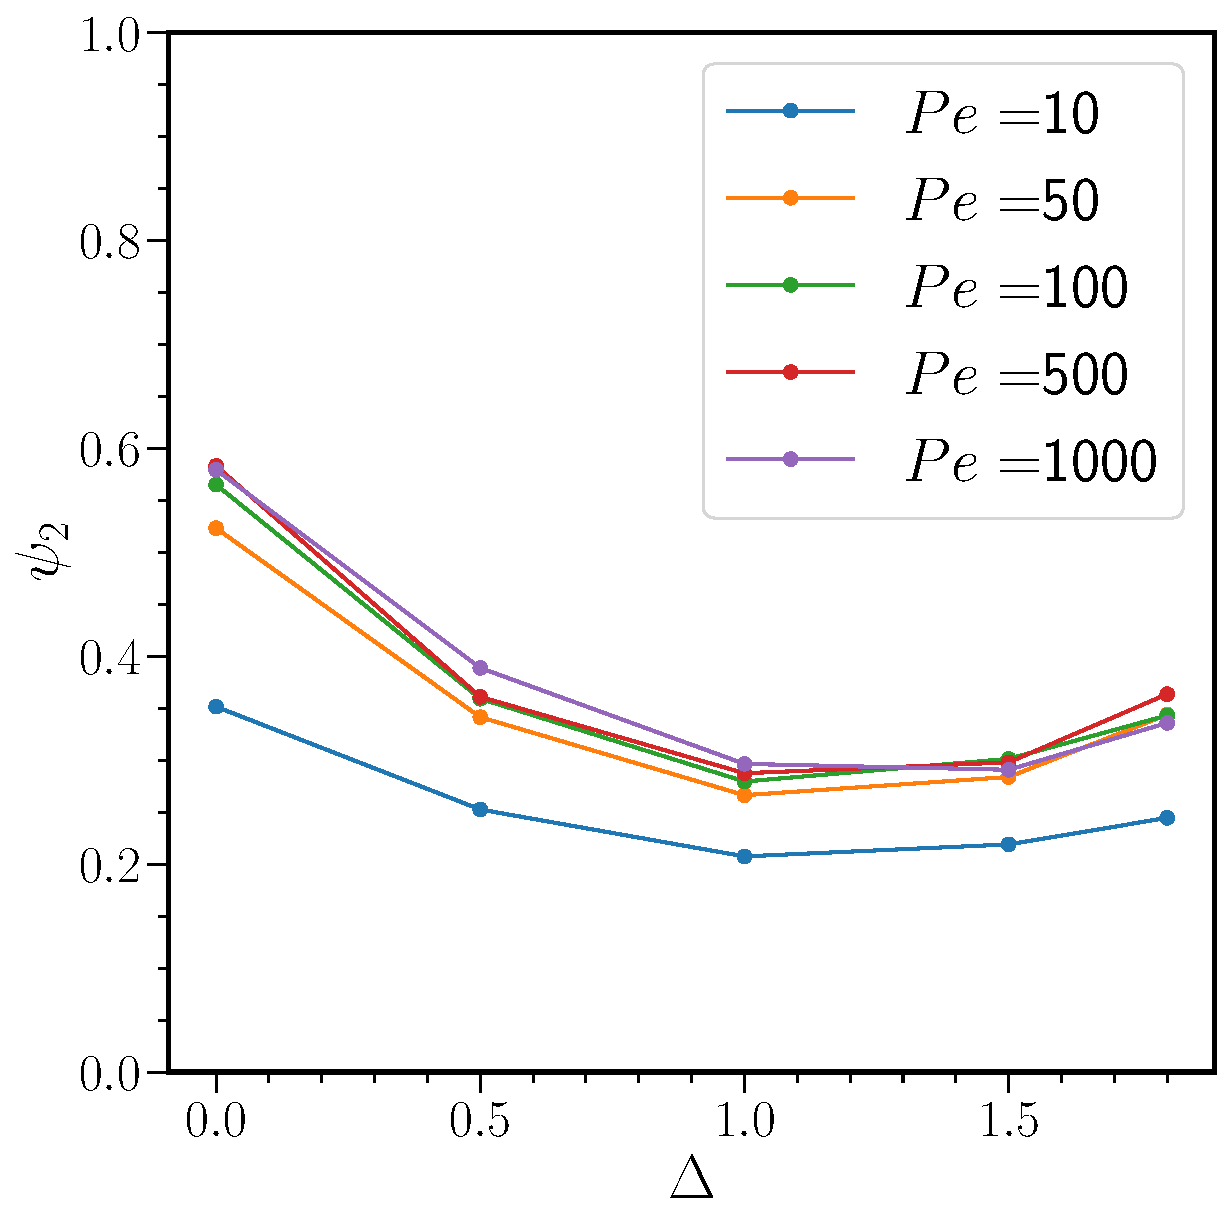
\includegraphics[width=\textwidth]{img/bit/ani_test/psi_20.70.110.pdf}
        \end{minipage}
        % \begin{minipage}{0.3\hsize}
        %     \text{(b)}
        %     \includegraphics[width=\textwidth]{img/bit/ani_test/L_{z2}0.70.110.pdf}
        % \end{minipage}
        \begin{minipage}{0.4\hsize}
            \text{(b)}
            \includegraphics[width=\textwidth]{img/bit/ani_test/V_{2}0.70.110.pdf}
        \end{minipage}
    \end{tabular}
    \caption[two_hdlm]
    {
        $\varphi=0.7、R=10、M=0.1$
    }
    \label{fig:twocer_lo0.7_r10_m0.1}
\end{figure}
まず$Pe$依存性について見ると、$\psi_2、V_2$においてそれらの絶対値が大きくなっており、これは%TODO*ref\
と同様に$Pe$が大きくなると粒子が同じ方向へと流れ流ことがわかる。
次に$\Delta$依存性について見ると、$\Delta\simeq1.4$周りで$V_2$の符号が正から負へと変化しており、
これは$\Delta$を大きくすると2つの円の流れが同じ方向から逆の流れへと変化する。
% これ以上何を言う?
\end{document}
